\section{Dataset and Preprocessing}
\textbf{Owner: Rifnaz.K.R.M -- 230550P}

The dataset used in this project is DeFungi from the UCI Machine Learning Repository \cite{defungi_uci}. It contains microscopic fungi images belonging to five classes: H1, H2, H3, H5, and H6. The verified local dataset contains 9,114 usable RGB JPEG images. No unreadable images were found during dataset verification.

\begin{table}[H]
\centering
\caption{Verified class distribution.}
\label{tab:class_distribution}
\begin{tabular}{lr}
\toprule
Class & Images \\
\midrule
H1 & 4,404 \\
H2 & 2,334 \\
H3 & 819 \\
H5 & 818 \\
H6 & 739 \\
\midrule
Total & 9,114 \\
\bottomrule
\end{tabular}
\end{table}

\begin{figure}[H]
\centering
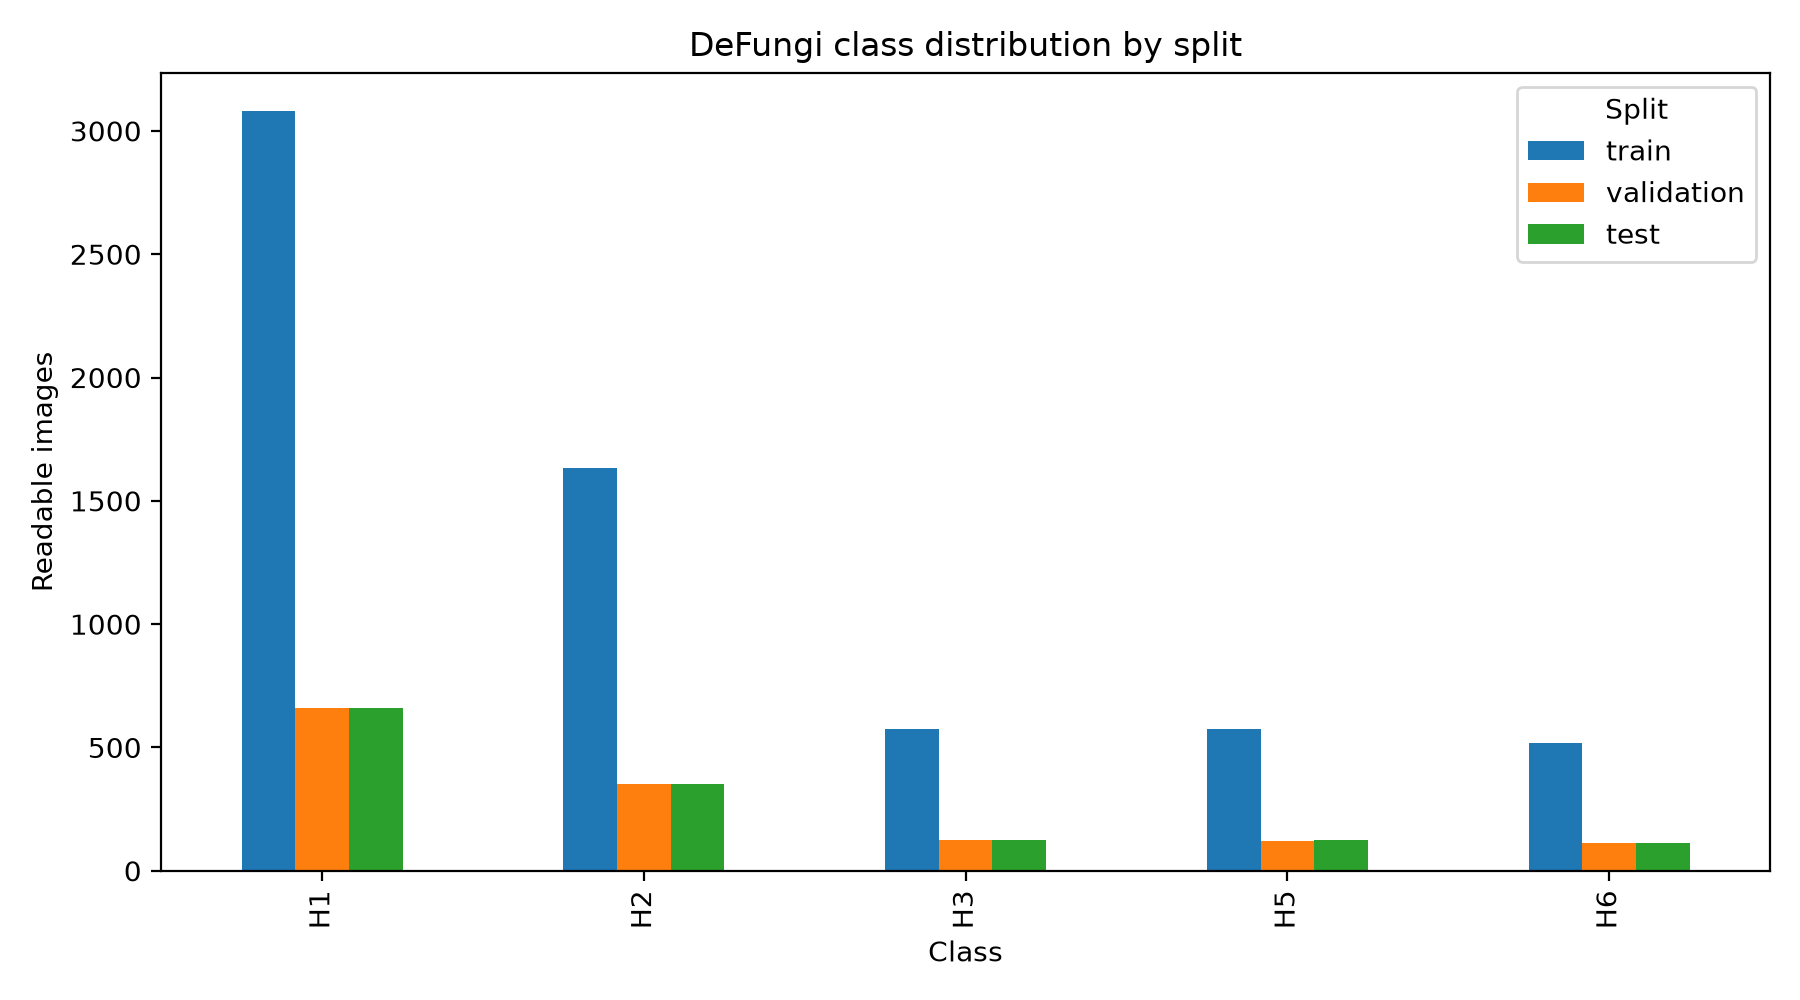
\includegraphics[width=0.72\linewidth]{figures/class_distribution.png}
\caption{Class distribution of the verified DeFungi dataset.}
\label{fig:class_distribution}
\end{figure}

The data split was created once and reused for all experiments. A stratified 70/15/15 target split was used with seed 42, giving 6,379 training images, 1,367 validation images, and 1,368 test images. The class membership of the validation and test sets is therefore fixed across custom and pretrained models.

\begin{table}[H]
\centering
\caption{Verified stratified split counts.}
\label{tab:split_counts}
\begin{tabular}{lrrrrrr}
\toprule
Split & H1 & H2 & H3 & H5 & H6 & Total \\
\midrule
Train & 3,082 & 1,634 & 573 & 573 & 517 & 6,379 \\
Validation & 661 & 350 & 123 & 122 & 111 & 1,367 \\
Test & 661 & 350 & 123 & 123 & 111 & 1,368 \\
\bottomrule
\end{tabular}
\end{table}

For the custom CNNs, all images were resized to $64 \times 64 \times 3$ and pixel values were normalized to the range $[0,1]$. For the pretrained models, images were resized to $224 \times 224 \times 3$ and processed with the corresponding Keras application preprocessing functions.
